Figure~\ref{fig:4:fw} in Chapter~\ref{chap:cc.fw} shows the structure of the
congestion control framework described in this thesis. The framework
categorizes \emph{In-path} sources and \emph{out-of-band} signaling for
implementing congestion control, which are discussed in this chapter. This
chapter is based on our work on Multipath RTP (MPRTP), which is documented in
\citepub{c:mprtp}, in \cite{draft.mprtp}, \cite{draft.mprtp.sdp},
\cite{Globisch:AsymGrpComm}, and \cite{draft.rtcp.overlay}.

In \citepub{c:mprtp}, we propose the following: design goals of implement a
multipath protocol for multimedia, protocol details, scheduling algorithm to
send media packets over multiple paths, a dejitter buffer implementation to
playout packets smoothly even when the path skew is high. We evaluate the
performance of the proposed mechanisms in diverse scenarios in our testbed.
Lastly, we discuss the system consideration for deployment.

\section{Multipath RTP (MPRTP)}

The Internet backbone has evolved over the past decades to a mesh of service
providers with manifold peerings that are generally capable of offering a
number of (independent) paths between two nodes. Networks often use multiple
attachment points for resilience purposes, such as data enterprise networks or
data centers and even routers for SOHO networks support multiple access
networks~\cite{draft.fun.multi, draft.homenet.arch}. Additionally, many hosts
today feature multiple network interfaces (e.g., WLAN and 3G on mobile
devices), this may yield the possibility for two endpoints to communicate via
multiple paths. While exploiting multipath characteristics
\cite{Wischik:2008:RPP} has been explored for TCP (e.g.,
MPTCP)~\cite{rfc6824}, the requirements for real-time traffic differs notably
and TCP can only serve real-time communication within tight constraints of
network characteristics~\cite{Brosh:tcp-real-time}. In the multipath case, the
scheduling algorithms do not consider real-time bounds when spreading data
segments across different paths and diverse paths may lead to worst case delay
and thus even longer buffering time.


We propose Multipath RTP (MPRTP) as a backwards compatible extension to
RTP~\cite{rfc3550}, it is documented in \cite{draft.mprtp} and defines the
basic mechanisms to operate across multiple parallel paths.
Figure~\ref{chap7:fig_mprtp} shows a macroscopic system overview of MPRTP. The
primary use-case for MPRTP is transporting media flows between multi-homed
endpoints. Such endpoints could be residential IPTV or telepresence devices
that connect to the Internet through two different Internet service providers
(ISPs), or mobile devices that connect to the Internet through 3G and WLAN
interfaces. By allowing RTP to use multiple paths for transmission, the
following gains can be achieved:

\begin{enumerate}
\setlength{\itemsep}{5pt}

\item \textbf{\texttt{Higher quality}}: Pooling the resource capacity of
multiple Internet paths allows higher bit-rate and higher quality codecs to be
used. From the application perspective, the available bandwidth between the
two endpoints increases.

\item \textbf{\texttt{Load balancing}}: Transmitting an RTP stream over
multiple paths reduces the bandwidth usage on a single path, which in turn
reduces the impact of the media stream on other traffic on that path. Also by
seamlessly offloading a flow from one path to another allows for some gains,
for example, reduces energy consumption, reduces access costs, or reduces
network latency.

\item \textbf{\texttt{Fault tolerance}}: Using multiple paths in conjunction
with redundancy mechanisms (FEC, re-transmissions, etc.), outages on one path
have less impact on the overall perceived quality of the stream. This can also
enable seamless handover in the case of mobility, i.e., moving from one
network to another.

\end{enumerate}


\begin{figure}
\centerline {
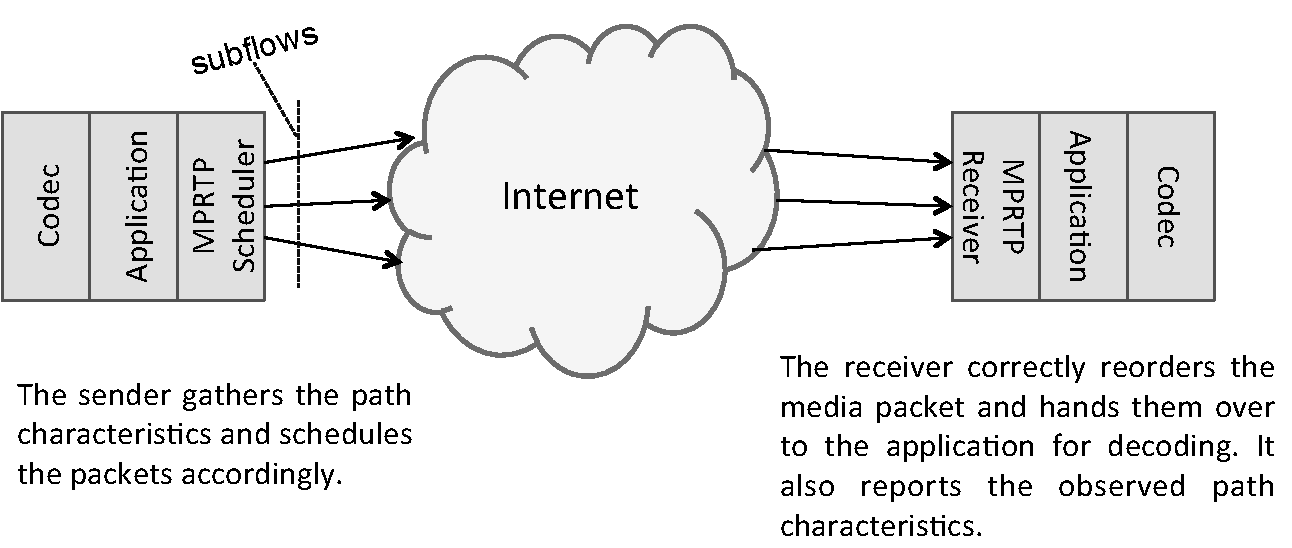
\includegraphics[width=0.9\textwidth]{chap7-fig_mprtp-1}
}
\caption{System Overview: A sender uses multiple paths to stream media
  to a receiver.  The receiver uses a dejitter buffer to reorder
  packets and sends per-path characteristics to the sender that
  distributes the packets based on the reported values.}
\label{chap7:fig_mprtp}
\end{figure}

The design goals for MPRTP from our perspective are: MPRTP-enabled system to
be able to make use of multiple paths and adapt to their relative capacity
changes by redistributing the load. As different paths will likely exhibit
different RTTs, mechanisms must be developed to overcome the resulting skew.
Furthermore, the choice of suitable transmission paths should reflect the
demands of the application. From a protocol perspective, RTP must be extended
to perform these functions, yet maintain backwards compatibility.
